\newpage
\hypertarget{checkCard vis}{}
\subsection{Implementing check}
\visHeader

\begin{itemize}

\vspace{1cm}

\item[$\blacktriangleright$] Since you're nearly an SDM wizard already, try using concepts we have already learnt to create the control flow for
\texttt{Partition::check} as depicted in Fig.~\ref{fig:sdm_check_start}.

\vspace{1cm}

\begin{figure}[htbp]
\begin{center}
  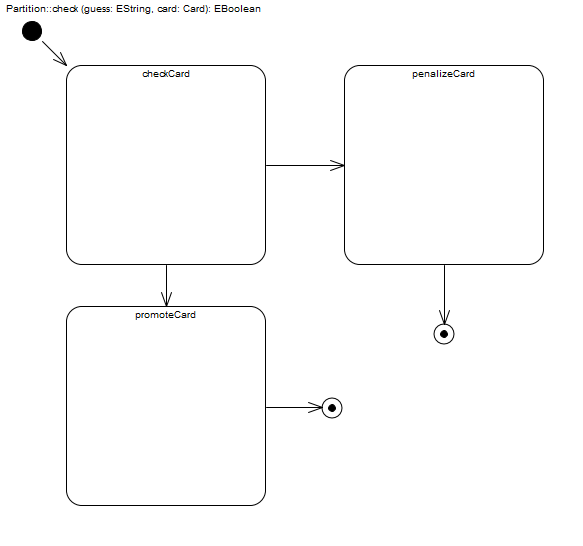
\includegraphics[width=0.9\textwidth]{ea_activityCheck}
  \caption{Activity diagram for \texttt{Partition::check}}
  \label{fig:sdm_check_start}
\end{center}
\end{figure}

\vspace{1cm}

\item[$\blacktriangleright$] In \texttt{checkCard}, create an object variable that is bound to the parameter argument, \texttt{card} 
(Fig.~\ref{fig:sdm_check_addCard}). This will represent the card the user picked from the learning box. Remember, the binding for this variable is implicitly
defined because its name is the same as the argument's.

\begin{figure}[htbp]
\begin{center}
  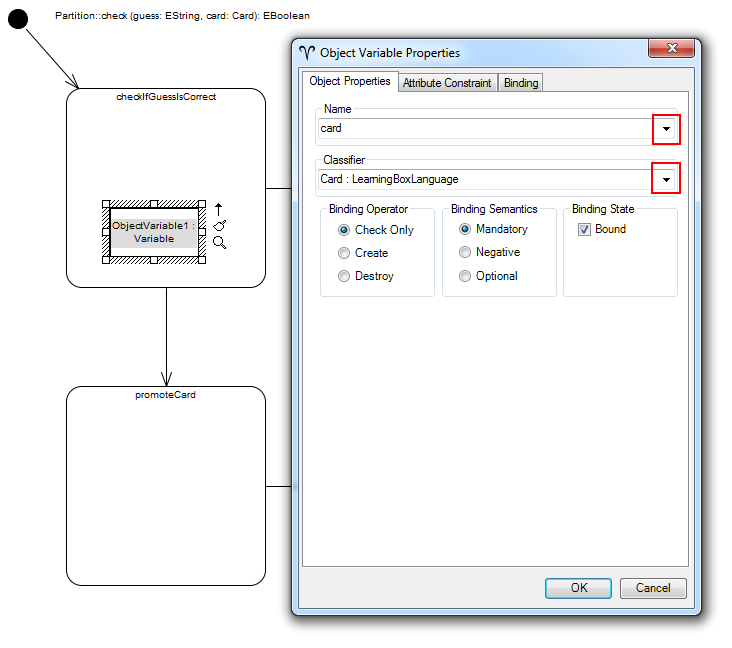
\includegraphics[width=\textwidth]{ea_addObjVarCard}
  \caption{Creating the card variable}
  \label{fig:sdm_check_addCard}
\end{center}
\end{figure}

\clearpage

\item[$\blacktriangleright$] Now that the pattern has the correct card to check, it needs to compare the user's guess against the unseen \texttt{face} value on
the opposite side. To do this, we need to specify an \emph{attribute constraint}. Open the \texttt{attribute constraint} tab for \texttt{card} as depicted in
Fig.~\ref{fig:sdmcheck_att_constraint}, and select the correct \texttt{Attribute} and \texttt{Operator}.

\vspace{0.5cm}

\begin{figure}[htbp]
\begin{center}
  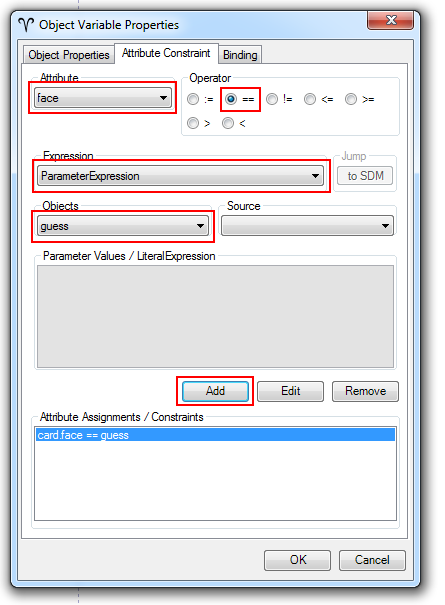
\includegraphics[width=0.6\textwidth]{ea_addAttConst}
  \caption{Creating an attribute constraint}
  \label{fig:sdmcheck_att_constraint}
\end{center}
\end{figure}

\item[$\blacktriangleright$] Similar to how the return value was specified in the previous SDM, set the \texttt{ParameterExpression} to refer to \texttt{guess},
i.e., the user's EString input. Press \texttt{Add}, and admire your first conditional.

\end{itemize}

Before building the other two activity nodes, let's quickly return to the control flow. Currently, the pattern branches off into two separate patterns after
completing the initial check, and it is unclear how to terminate the method. As the code generator does not know what to do here, this is flagged as a
validation error (you're free to press the validation button and take cover) We need to add \emph{edge guards}\define{Edge Guards} to change this into an
\emph{if/else} construct based on the results of the \emph{attribute constraint}.

\newpage
\begin{itemize}

\item[$\blacktriangleright$] To add a guard to the edge leading from \texttt{check\-If\-Guess\-Is\-Correct} to \texttt{penalize\-Card}, double click the edge
and set the \emph{Guard Type} to \texttt{Failure} (Fig.~\ref{fig:sdm_check_guard}). Repeat the process for the \texttt{Success} edge leading to
\texttt{promoteCard}.

\vspace{0.5cm}

\begin{figure}[htbp]
\begin{center}
  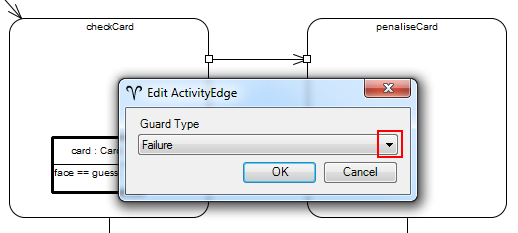
\includegraphics[width=0.75\textwidth]{ea_addTransitionGuard}
  \caption{Add a transition with a guard}
  \label{fig:sdm_check_guard}
\end{center}
\end{figure}

\vspace{0.5cm}

\end{itemize}

One great feature of eMolfon (with EA) is a means of coping with large patterns. It might be nice to visualise \emph{small} story patterns directly in their
nodes (such as \texttt{removeCardFromPartition}), but for large patterns or complex control flow, such diagrams would get extremely cumbersome and unwieldy
\emph{very} quickly! This is indeed a popular argument against visual languages and it might have already crossed your mind -- ``This is cute, but it'll
\emph{never} scale!'' With the right tools and concepts however, even huge diagrams can be mastered. eMoflon supports \emph{extracting} story patterns into
their own diagrams, and unless the pattern is really concise with only 2 or 3 object variables, we recommend this course of action. In other words, eMoflon
supports separating your transformation's pattern layer from its imperative control flow layer.


\begin{itemize}

\item[$\blacktriangleright$] To try this, double-click the \texttt{promoteCard} story node and choose \texttt{Extract Story Pattern}
(Fig.~\ref{fig:sdm_check_extract_storypattern}). Note the new diagram that is immediately created and opened in the project browser
(Fig.~\ref{fig:sdm_new_sub_diagram}).

\begin{figure}[htbp]
\begin{center}
  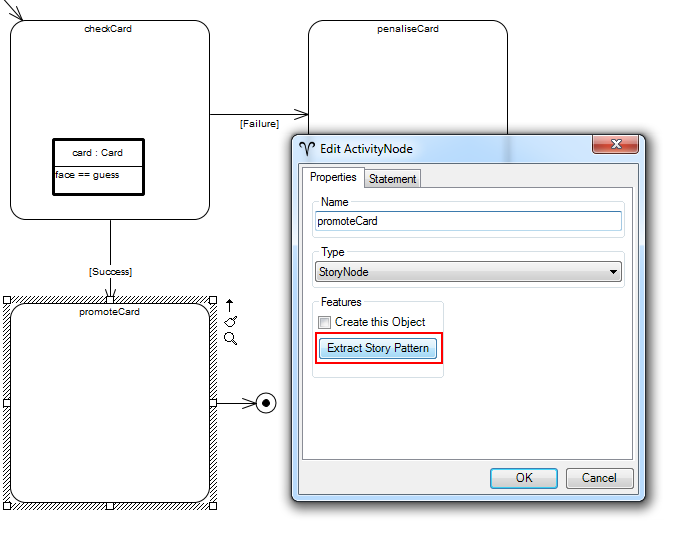
\includegraphics[width=0.8\textwidth]{ea_extractStoryPattern}
  \caption{Extract a story pattern for more space and a better overview}
  \label{fig:sdm_check_extract_storypattern}
\end{center}
\end{figure}

\begin{figure}[htbp]
\begin{center}
  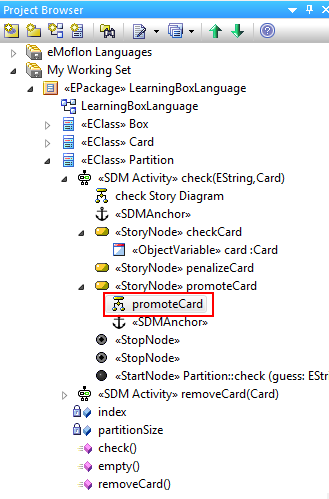
\includegraphics[width=0.45\textwidth]{sdm_promoteCardProjBrowser}
  \caption{A new subdiagram is created automatically}
  \label{fig:sdm_new_sub_diagram}
\end{center}
\end{figure}

\newpage

Another EA gesture\footnote{The other two gestures we have learnt are ``Quick Link'' and ``Quick Create''} you could start to take advantage of here is good
ol' \emph{Drag-and-Drop} from the project browser into a diagram. We can use this action as an alternative to creating new objects (with known types) from
the SDM toolbox.

The main advantage of drag-and-drop is that the \texttt{Object Variable Pro\-per\-ties} dialogue will have the type of the object pre-configured. Choosing
the type in the project browser and dragging it in is (for some people) a more natural gesture than choosing the type from a long drop-down menu (as we had to
when using the SDM toolbar). This can be a great time saver for large metamodels.\footnote{Drag-and-drop is also possible in embedded story patterns
(those still visualised in their story nodes).  You must ensure however, that the object variable is \emph{completely} contained inside the story node, and does
not stick out over any edge.}

\vspace{0.5cm}

\item[$\blacktriangleright$] To put this into practice, create a new \texttt{Card} object variable by drag-and-dropping the class from the project browser
into the new (extracted) pattern diagram (Fig.~\ref{fig:sdm_check_bound_card}).

\vspace{0.5cm}

\begin{figure}[htbp]
\begin{center}
  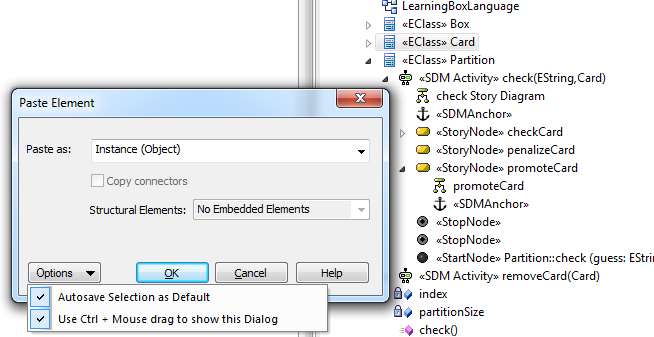
\includegraphics[width=\textwidth]{ea_dragDropDialogue}
  \caption{Add a new object variable per drag-and-drop}
  \label{fig:sdm_check_bound_card}
\end{center}
\end{figure}

\item[$\blacktriangleright$] A dialogue will appear asking what kind of visual element should be created. You can create (1) a simple link (which would refer to
and be represented by the class \texttt{Card}), (2) create an instance of \texttt{Card} as an object variable, or (3) as an invocation (which has no meaning
for eMoflon diagrams). Paste \texttt{Card} as an \texttt{Instance}, and select \texttt{Autosave Selection as Default} under ``Options" so option (2) will be
used next time by default. You should also select \texttt{Use Ctrl + Mouse drag to show this Dialog}, so this dialogue doesn't appear every time you use this
gesture. Don't worry -- if you ever need option (1), hold \texttt{Ctrl} when dragging to invoke the dialogue again.

\vspace{0.5cm}

\item[$\blacktriangleright$] After creating the object, the object properties dialogue will open.  Set the \texttt{Name} to \texttt{card} and confirm its
\texttt{Binding State} is \texttt{Bound} (Fig.~\ref{fig:sdm_new_card_properties}).

\begin{figure}[htbp]
\begin{center}
  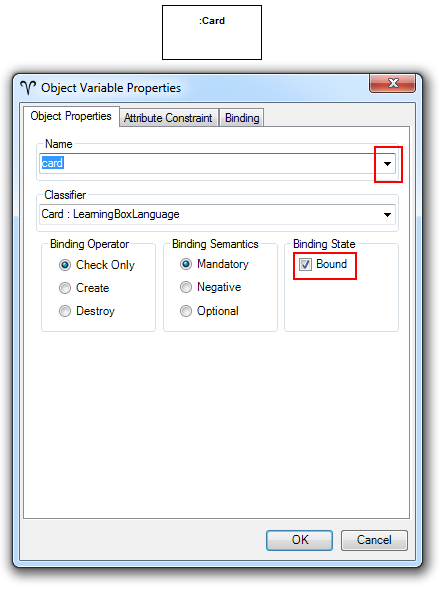
\includegraphics[width=0.5\textwidth]{ea_addBoundObj}
  \caption{Object variable properties of the new card}
  \label{fig:sdm_new_card_properties}
\end{center}
\end{figure}

\vspace{0.5cm}

\item[$\blacktriangleright$] Currently, we have the single \texttt{card} that we want to promote through the box. Drag-and-drop two partition objects,
\texttt{this}, and \texttt{nextPartition} as depicted in Fig.~\ref{fig:sdm_check_complete_sp}.

\vspace{0.5cm}

\begin{figure}[htbp]
\begin{center}
  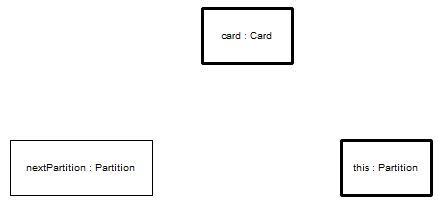
\includegraphics[width=0.8\textwidth]{ea_promoteCardVariables}
  \caption{All object variables for story pattern \texttt{promoteCard}}
  \label{fig:sdm_check_complete_sp}
\end{center}
\end{figure}

An important point to note here is that \texttt{this} and \texttt{card} are visually differentiated from \texttt{nextPartition} by
their bold border lines. This is how we differentiate \emph{bound} from \emph{unbound} (\emph{free}) variables. We already know that matches for bound
variables are completely determined by the current context. On the other hand, matches for unbound variables have to be determined by the pattern matcher. Such
matches are ``found'' by navigating and searching the current model for possible matches that satisfy all specified constraints (i.e., type of the variable,
links connecting it to other variables, and attribute constraints). In our case, \texttt{nextPartition} should be determined by navigating from
\texttt{this} via the \texttt{next} link variable.

\vspace{0.5cm}

\item[$\blacktriangleright$] To specify this, quick link from \texttt{this} to \texttt{nextPartition} (or vice-versa) to establish
\texttt{next}, as shown in Fig.~\ref{fig:sdm_check_link_variable}. As you can see, there are several more options than what was seen in
\texttt{removeCard}. The goal is to have the current partition to proceed (or point) to the \texttt{nextPartition} via the \texttt{next} reference, so select
the second option. Alternatively, you could define the reference from \texttt{nextPartition} by setting the link variable \texttt{previous} to \texttt{this}.

\begin{figure}[htbp]
\begin{center}
  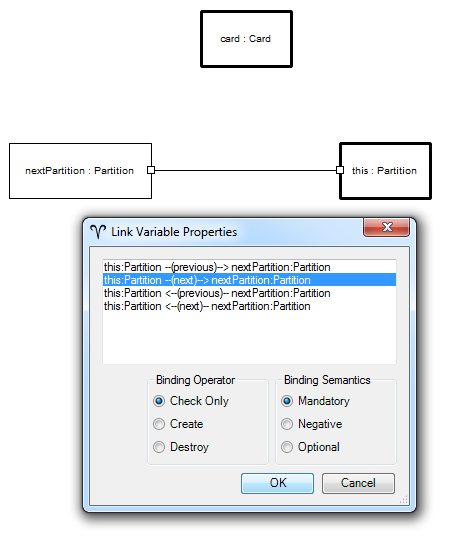
\includegraphics[width=0.85\textwidth]{ea_promoteLinkProperties}
  \caption{Possible links between \texttt{this} and \texttt{nextPartition}}
  \label{fig:sdm_check_link_variable}
\end{center}
\end{figure}

\vspace{0.5cm}

\item[$\blacktriangleright$] Continue by creating links between \texttt{card} and each partition. Remember - you want to \emph{destroy} the reference to
\texttt{this}, and \emph{create} a new connection to \texttt{nextPartition}. If everything is set up correctly, \texttt{promoteCard} should now closely resemble
Fig.~\ref{fig:sdm_check_complete_activity_node}.

\begin{figure}[htbp]
\begin{center}
  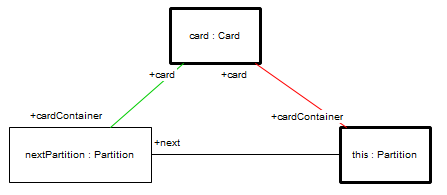
\includegraphics[width=0.8\textwidth]{ea_promoteCardCompleted}
  \caption{Complete story pattern for \texttt{promoteCard}}
  \label{fig:sdm_check_complete_activity_node}
\end{center}
\end{figure}

\clearpage

\item[$\blacktriangleright$] Double click the anchor in the top left corner and repeat the process for \texttt{penalizeCard}: First extract the story pattern,
then create the necessary variables and links as depicted in Fig.~\ref{fig:sdm_check_complete_penalize}. As you can see, this pattern is nearly identical to
\texttt{promoteCard}, except it moves \texttt{card} to a \texttt{previousPartition}.

\vspace{0.5cm}

\begin{figure}[htbp]
\begin{center}
  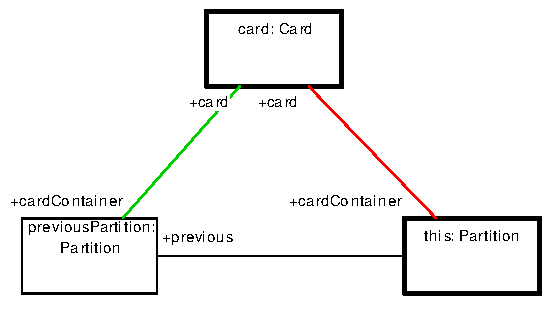
\includegraphics[width=0.8\textwidth]{ea_completeActivityPenalize.pdf}
  \caption{Complete story pattern for \texttt{penalizeCard}}
  \label{fig:sdm_check_complete_penalize}
\end{center}
\end{figure}


\vspace{0.5cm}

To complete the \texttt{check} activity, we need to signal (as a return value) the result of the check - was the card promoted or penalized? We have no object
to return so instead, we need to edit the stop nodes so they return a \emph{LiteralExpression}\define{LiteralExpression}. This expression type can be used to
specify arbitrary text, but should really only be used for true literals like 42, ``foo'' or \texttt{true}. It can be (mis)used for formulating any (Java)
expression that will simply be transferred ``literally'' into the generated code, but this is obviously really dirty\footnote{It defeats, for example, any
attempt to guarantee type safety} and should be avoided when possible.

\vspace{0.5cm}

\item[$\blacktriangleright$] To implement a literal, double click the stop node stemming from  \texttt{promoteCard}, and change the expression type from
\texttt{void} to \texttt{LiteralEx\-pression} (Fig.~\ref{fig:sdm_check_literal_exp}). Change the value in the window below to \texttt{true}. Press \texttt{OK},
then finish the SDM by returning \texttt{false} after \texttt{penalizeCard} in the same manner. Your diagram should now resemble
Fig.~\ref{fig:sdm_check_finish}.

\begin{figure}[htbp]
\begin{center}
  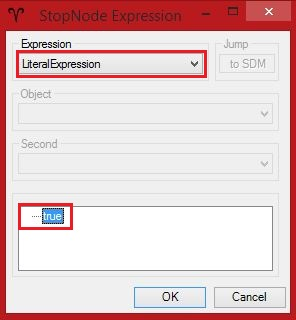
\includegraphics[width=0.5\textwidth]{ea_stopNodeLiteral}
  \caption{Add a return value with a literal expression}
  \label{fig:sdm_check_literal_exp}
\end{center}
\end{figure}

\begin{figure}[htbp]
\begin{center}
  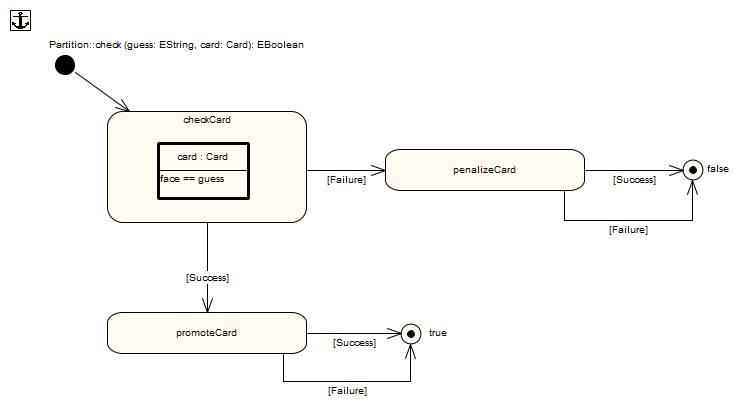
\includegraphics[width=\textwidth]{ea_sdmCheckComplete}
  \caption{Complete SDM for \texttt{Partition::check}}
  \label{fig:sdm_check_finish}
\end{center}
\end{figure}

\clearpage

\item[$\blacktriangleright$] Great job -- the SDM is now complete! Validate and export your project, then inspect the implementation code for \texttt{check}. We
strongly recommend that you even write a simple JUnit test (take a look at our simple test case from Part I for inspiration) to take your brand new SDM for a
test-spin.

\item[$\blacktriangleright$] To see how this is implemented in the textual syntax, see Figs. \ref{fig:completedPatterns} and \ref{fig:finalMethod} in the
following section.

\jumpSingle{sec:extendGui}

\end{itemize}
